\documentclass[12pt]{article}
\usepackage[a4paper,margin=20mm,top=19mm,bottom=20mm]{geometry}
\usepackage[T1]{fontenc}
\usepackage{lmodern,microtype,amsmath,amssymb,booktabs,array}
\usepackage[most]{tcolorbox}
\usepackage{tikz,fancyhdr,hyperref}
\usetikzlibrary{arrows.meta,positioning,calc}
\definecolor{ink}{HTML}{182B3A}
\definecolor{teal}{HTML}{007F86}
\definecolor{orange}{HTML}{B96117}
\definecolor{purple}{HTML}{6A4C93}
\definecolor{muted}{HTML}{637381}
\color{ink}
\hypersetup{colorlinks=true,linkcolor=teal,urlcolor=teal,pdftitle={IRMF: the proof in five steps},pdfauthor={IMF research project},bookmarksopen=true}
\setlength{\parindent}{0pt}
\setlength{\parskip}{8pt}
\setlength{\headheight}{15pt}
\setlength{\footskip}{23pt}
\linespread{1.04}
\emergencystretch=2em
\pagestyle{fancy}\fancyhf{}
\fancyhead[L]{\sffamily\small\color{muted}IRMF / the proof in five steps}
\fancyhead[R]{\sffamily\small\color{muted}Proposition 4.1 to all components}
\fancyfoot[R]{\sffamily\small\thepage\,/\,5}
\renewcommand{\headrulewidth}{.3pt}
\newcommand{\page}[3]{\clearpage\phantomsection\pdfbookmark[0]{#2}{p#1}{\sffamily\color{teal}\small #1\quad /\quad #3}\par\vspace{4pt}{\sffamily\bfseries\LARGE #2}\par\vspace{5pt}}
\newcommand{\sub}[1]{\par\vspace{4pt}{\sffamily\bfseries\large #1}\par}
\newcommand{\captiontext}[1]{{\small\color{muted}#1}\par}
\newcommand{\norm}[1]{\left\|#1\right\|_\infty}
\newtcolorbox{takeaway}{colback=teal!5,colframe=teal!65,boxrule=.6pt,arc=1.5mm,left=11pt,right=11pt,top=9pt,bottom=9pt,before skip=10pt,after skip=9pt}
\newtcolorbox{caution}{colback=orange!5,colframe=orange!65,boxrule=.6pt,arc=1.5mm,left=11pt,right=11pt,top=9pt,bottom=9pt,before skip=10pt,after skip=9pt}
\tikzset{card/.style={draw=teal!55,fill=teal!4,rounded corners=3pt,align=center,font=\small,inner sep=7pt,minimum height=15mm},arrow/.style={-{Stealth[length=2.3mm]},thick,draw=muted}}
\begin{document}

\page{01}{One fit: score divided by curvature}{The notation of Proposition 4.1}
At position $t$, fit $Y_u=X_u+\varepsilon_u$ using loss $\rho$ and local weights
$w_u\ge0$. To measure noise-induced error, we need a target fixed across samples.
Averaging the loss over noise gives $\phi(a)=\mathbb E\rho(a+\varepsilon)$ and
the population target below.
\begin{center}
\renewcommand{\arraystretch}{1.5}
\begin{tabular}{@{}lcc@{}}
\toprule
 & Population & Empirical\\
\midrule
Objective & $f(s)=\sum_u\phi(X_u-s)w_u$ & $f_\circ(s)=\sum_u\rho(Y_u-s)w_u$\\
Minimizer & $S_t=\arg\min f$ & $\widetilde S_t=\arg\min f_\circ$\\
\bottomrule
\end{tabular}
\end{center}
\captiontext{The proof also writes $x^*=S_t$ and $x_\circ=\widetilde S_t$.
The circle marks an empirical quantity.}

\sub{Why look at the score?}
The random minimizer is implicit. Evaluating the score at the fixed target
$S_t$ exposes the noise as a sum we can bound:
\[
 \nabla_t=-f_\circ'(S_t)
 =\sum_u\{\rho'(Y_u-S_t)-\mathbb E\rho'(Y_u-S_t)\}w_u.
\]
Subtracting each summand's expectation centers it; the total is unchanged because
$f'(S_t)=0$. Independence then permits concentration. Curvature $F_t=f''(S_t)>0$
is the expected score decrease per unit displacement, which explains the ratio
$\nabla_t/F_t$.
\begin{takeaway}
\[
 \widetilde S_t-S_t
 =\underbrace{F_t^{-1}\nabla_t}_{\text{Fisher leading term}}
  +\underbrace{R_t}_{\text{single-pass remainder}}.
\]
The split isolates a noise term we can analyze. We then need to prove that
the leftover $R_t$ is smaller.
\end{takeaway}

\begin{center}
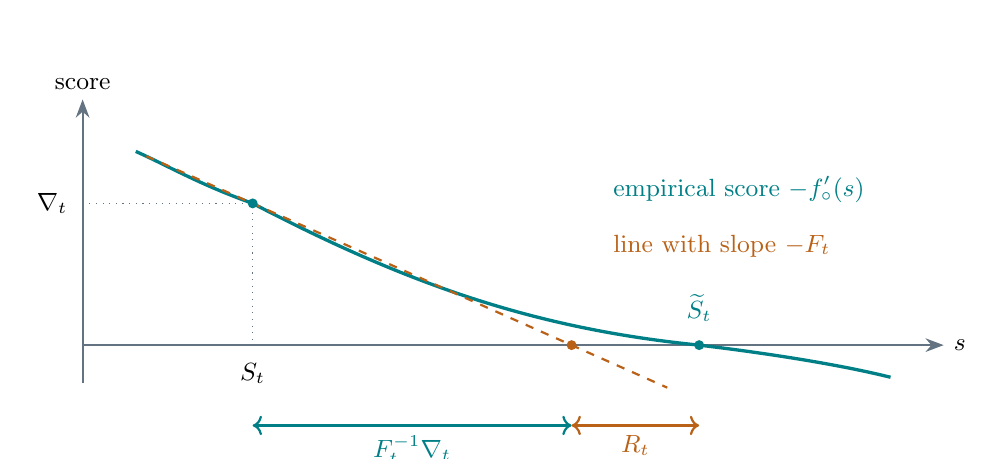
\begin{tikzpicture}[x=1.35cm,y=1.2cm,font=\small]
\draw[arrow] (.4,0)--(8.5,0) node[right] {$s$};
\draw[arrow] (.4,-.4)--(.4,2.6) node[above] {score};
\draw[teal,very thick] (.9,2.05) .. controls (1.2,1.9) and (1.5,1.7) .. (2,1.5)
 .. controls (3.4,.68) and (4.6,.18) .. (6.2,0)
 .. controls (6.8,-.08) and (7.5,-.2) .. (8,-.34);
\draw[orange,thick,dashed] (1,2.0)--(5.9,-.45);
\draw[muted,dotted] (.4,1.5)--(2,1.5)--(2,0);
\node[anchor=east] at (.35,1.5) {$\nabla_t$};
\fill[teal] (2,1.5) circle (1.8pt);
\fill[orange] (5,0) circle (1.8pt);
\fill[teal] (6.2,0) circle (1.8pt);
\node[below=3pt] at (2,0) {$S_t$};
\node[above=5pt,teal] at (6.2,0) {$\widetilde S_t$};
\node[teal,anchor=west] at (5.3,1.65) {empirical score $-f_\circ'(s)$};
\node[orange,anchor=west] at (5.3,1.05) {line with slope $-F_t$};
\draw[<->,teal,thick] (2,-.85)--node[below] {$F_t^{-1}\nabla_t$}(5,-.85);
\draw[<->,orange,thick] (5,-.85)--node[below] {$R_t$}(6.2,-.85);
\end{tikzpicture}
\end{center}
\captiontext{Schematic. The line predicts the displacement; $R_t$ is its error.
Its sign can be either positive or negative.}

Subtract $F_t^{-1}\nabla_t$ to remove the leading noise effect.

\page{02}{What the single-pass proof controls}{Newton error and curvature fluctuation}
Taylor expansion follows the actual objective, so its first step uses the
\emph{empirical} curvature $F_\circ=f_\circ''(S_t)$:
\[
 0=f_\circ'(\widetilde S_t)
 \approx-\nabla_t+F_\circ(\widetilde S_t-S_t).
\]
We replace $F_\circ$ by $F_t$ to leave all randomness in the centered score.
The deterministic denominator preserves the sum structure needed for concentration
and for propagating leading terms through later stages. The replacement has a cost:
\begin{takeaway}
\begin{align*}
 R_t={}&\underbrace{\widetilde S_t-S_t-F_\circ^{-1}\nabla_t}_{\text{Newton error: curvature changes along the move}}\\[8pt]
 &+\underbrace{(F_\circ^{-1}-F_t^{-1})\nabla_t}_{\text{curvature fluctuation: empirical versus population}}.
\end{align*}
\end{takeaway}

\sub{Why both errors are second order}
The Newton error is quadratic in the displacement when the third derivative
is bounded and curvature stays positive. The replacement error multiplies
score fluctuation by curvature fluctuation:
\[
 \left|(F_\circ^{-1}-F_t^{-1})\nabla_t\right|
 =\frac{|F_\circ-F_t|\,|\nabla_t|}{F_\circ F_t}.
\]
Lemma 4.2 bounds these fluctuations on one high-probability event.
The convexity and smallness conditions keep the fit in the neighborhood where
Taylor's estimate holds. Without that localization, a small score at $S_t$
would not by itself justify the expansion at the minimizer.

\sub{Why scale by the square root of curvature?}
The same displacement costs more loss in a steeper objective. Locally,
$f(s)-f(S_t)\approx\tfrac12F_t(s-S_t)^2$.
Thus $D_t=\sqrt{F_t}$ puts displacements on a common quadratic-loss scale.
The proposition bounds
\[
 \left|D_t\bigl(\widetilde S_t-S_t-F_t^{-1}\nabla_t\bigr)\right|
 =D_t|R_t|.
\]

\begin{center}
\renewcommand{\arraystretch}{1.45}
\begin{tabular}{@{}lll@{}}
\toprule
Quantity & Role & Scale\\
\midrule
$F_t^{-1}\nabla_t$ & Leading noise effect & $\sqrt{z/m}$\\
$R_t$ & Error of the linear approximation & $z/m$\\
\bottomrule
\end{tabular}
\end{center}
The confidence cost $z$ pays for requiring the bounds at all positions and stages
at once. The effective window size $m=1/\max_u(w_u/\sum_vw_v)$ controls how much
one observation can influence the fit; it equals the window size for uniform
weights. The rates assume controlled curvature.

\page{03}{Carry the error into the next fit}{The same noise is reused}
Earlier fits make residual coordinates dependent. Run the $\phi$-recursion on
the clean signal to obtain deterministic input $X_\phi^{(k)}$ and component
$S_\phi^{(k)}$. The auxiliary input $X_\phi^{(k)}+\varepsilon$ then has independent
coordinates. Write the fit as $\mathcal M_k$ to compare its outputs on this input
and the actual residual. All earlier component errors were subtracted;
their sum $E_k$ enters as
\begin{takeaway}
\[
 \underbrace{Y^{(k)}}_{\text{actual input}}
 =\underbrace{X_\phi^{(k)}+\varepsilon}_{\text{reference plus original noise}}
  -\underbrace{E_k}_{\text{past errors}}.
\]
Proposition 4.1 applies to the unshifted input $X_\phi^{(k)}+\varepsilon$.
The propagation step accounts for the shift $-E_k$.
\end{takeaway}

To predict the effect of $E_k$, linearize the population fit with respect to its
inputs. Its deterministic response matrix $V_k$ averages errors with weights
proportional to expected curvature. Its rows sum to one. Define
\[
 \Phi_k=\mathcal M_k(X_\phi^{(k)}+\varepsilon)
       -\mathcal M_k(Y^{(k)})-V_kE_k.
\]
Thus $\Phi_k$ measures the error in predicting the change of fit by $V_kE_k$.
Writing $b_k$ for the single-pass Fisher term, the component error is exactly
\[
 e_k:=\mathcal M_k(Y^{(k)})-S_\phi^{(k)}
     =b_k-V_kE_k+R_k-\Phi_k.
\]

\sub{Why separate leading errors from remainders?}
The leading terms retain the centered-sum structure used for concentration.
The smaller remainder needs an inductive bound. Their accumulated sums match
what the next residual receives:
\begin{center}
\renewcommand{\arraystretch}{1.5}
\begin{tabular}{@{}lcc@{}}
\toprule
 & Current component & Sum of earlier components\\
\midrule
Total error & $e_k$ & $E_k=\sum_{j<k}e_j$\\
Leading term & $L_k$ & $\Lambda_k=\sum_{j<k}L_j$\\
Remainder & $Q_k=e_k-L_k$ & $\Theta_k=\sum_{j<k}Q_j$\\
\bottomrule
\end{tabular}
\end{center}
Initialize $\Lambda_1=\Theta_1=0$ and define the leading terms recursively:
\begin{takeaway}
\begin{align*}
 L_k&=\underbrace{b_k}_{\text{new noise effect}}
      -\underbrace{V_k\Lambda_k}_{\text{propagated leading errors}},\\[7pt]
 Q_k&=\underbrace{R_k}_{\text{single pass}}
      -\underbrace{\Phi_k}_{\text{propagation}}
      -\underbrace{V_k\Theta_k}_{\text{propagated remainders}}.
\end{align*}
\end{takeaway}
Thus $\Theta_k$ isolates the accumulated nonlinear error for the induction.
All stages still use the same original noise.

\page{04}{Control the propagation remainder}{Three forcing terms and one feedback term}
A Jacobian describes the response to an infinitesimal input change. Integrating
it along the shift from $X_\phi^{(k)}+\varepsilon$ to $Y^{(k)}$ gives the exact
finite change. Comparing it with $V_k$ separates four effects:
\begin{center}
\renewcommand{\arraystretch}{1.5}
\begin{tabular}{@{}p{100mm}l@{}}
\toprule
Source & Bound, up to constants\\
\midrule
Jacobian changes along the input movement & $\norm{E_k}^2$\\
Fitted Jacobian differs from the curvature matrix at the reference target
 & $\sqrt{z/m_k}\,\norm{E_k}$\\
Centered curvature multiplies past leading errors & $\norm{Z_k\Lambda_k}$\\
Centered curvature multiplies past remainders & $\norm{Z_k}\,\norm{\Theta_k}$\\
\bottomrule
\end{tabular}
\end{center}
\captiontext{$Z_k$ subtracts the mean from empirical curvature weights at the
reference target, using population curvature in the denominator. Centering
enables the cancellation below. The vector norm takes the worst error over
positions; the matrix norm is the largest absolute row sum.}

\sub{The third term needs cancellation}
$Z_k$ and $\Lambda_k$ depend on the same noise. Expand their product over pairs
of original observations \emph{before} taking absolute values. This preserves
centering and reveals which terms use independent observations.
\begin{center}
\begin{minipage}[c]{.29\linewidth}\centering
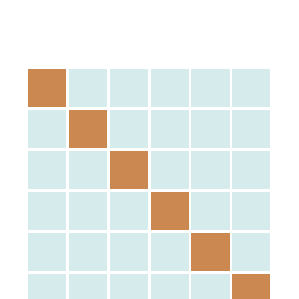
\begin{tikzpicture}[x=.52cm,y=.52cm]
\foreach \i in {0,...,5}{\foreach \j in {0,...,5}{\fill[teal!16] (\i,\j) rectangle ++(.93,.93);}}
\foreach \i in {0,...,5}{\fill[orange!75] (\i,5-\i) rectangle ++(.93,.93);}
\end{tikzpicture}
\end{minipage}\hfill
\begin{minipage}[c]{.67\linewidth}
\textcolor{orange}{Same observation.} The diagonal can have nonzero mean.
Bound it directly using the coefficient weights.

\textcolor{teal}{Different observations.} Centering and independence give zero
mean for each pair. A quadratic concentration bound controls their sum.
\end{minipage}
\end{center}
The result is $\norm{Z_k\Lambda_k}\lesssim z/m_k$ on the common probability event.
Zero expectation alone would not give this bound.

\sub{What is left for the induction}
The bound $\norm{E_k}\lesssim\sqrt{z/m_{k-1}}$ makes the first two terms
second order because earlier windows are wider. Therefore
\begin{takeaway}
\[
 \norm{\Phi_k}
 \lesssim\underbrace{z/m_k}_{\text{new forcing}}
       +\underbrace{\norm{Z_k}\,\norm{\Theta_k}}_{\text{feedback from past remainders}}.
\]
The first term is already bounded. The second carries the unknown past remainder
forward; the curvature-dispersion assumption limits how much returns as feedback.
\end{takeaway}
\captiontext{$m_k$ is the effective window size at stage $k$.
The symbol $\lesssim$ hides the fixed constants specified in the full theorem.}

\page{05}{Close the induction}{Control the accumulated remainder first}
Past remainders enter the next input through their sum $\Theta_k$.
This sum obeys a closed recursion; recover each component remainder afterward
by taking a difference:
\[
 \Theta_{k+1}=(I-V_k)\Theta_k+R_k-\Phi_k,\qquad \Theta_1=0.
\]
$I-V_k$ keeps the incoming error after subtracting the fit's linear response.
Unrolling preserves cancellation between stages inside the full product:
\begin{center}
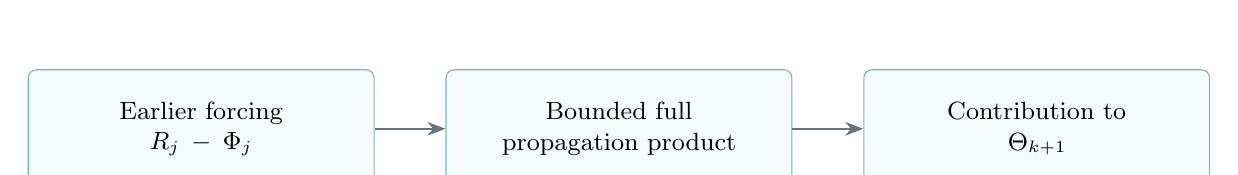
\begin{tikzpicture}
\node[card,text width=39mm] (a) {Earlier forcing\\$R_j-\Phi_j$};
\node[card,text width=39mm,right=9mm of a] (b) {Bounded full\\propagation product};
\node[card,text width=39mm,right=9mm of b] (c) {Contribution to\\$\Theta_{k+1}$};
\draw[arrow] (a)--(b);\draw[arrow] (b)--(c);
\end{tikzpicture}
\end{center}
Bounding the whole product prevents repeated worst-case amplification.
Geometrically shrinking windows give $\sum_{j\le k}m_j^{-1}\lesssim m_k^{-1}$, so earlier
forcing can be paid for at the current scale.

\sub{The closure inequality}
Assume $\norm{\Theta_j}\le Bz/m_{j-1}$ at earlier stages.
The preceding estimates give fixed $C,q$ such that
\begin{takeaway}
\[
 \norm{\Theta_{k+1}}\le(C+qB)\frac z{m_k}\le B\frac z{m_k}
 \quad\text{if}\quad q<1,\qquad B\ge\frac C{1-q}.
\]
$B$ is one allowance for every stage. Feedback uses $qB$ of that allowance;
$q<1$ leaves room for new forcing $C$. Dispersion, stability, and the geometric
window schedule determine $q$.
\end{takeaway}
The smallest window must also keep
$\norm{E_k}\le\norm{\Lambda_k}+\norm{\Theta_k}$ inside the local regime.
This sample-size condition validates the Taylor estimate used in the induction.
Finally,
\[
 Q_k=\Theta_{k+1}-\Theta_k,
 \qquad \norm{L_k}\lesssim\sqrt{z/m_k},
 \qquad \norm{Q_k}\lesssim z/m_k.
\]

\sub{Transfer to the paper's population target}
Our reference made independence usable. The paper's target instead averages
the loss of the actual residual, so we must also bound the distance between
these targets. Expand its expected score at $S_\phi^{(k)}$:
independence cancels the terms from different observations; diagonal and
remainder terms survive. Divide the resulting score bound by a lower curvature
bound to control the target shift.

Expectations include rare bad samples too; moment and tail conditions control
their contribution. Under those conditions the target shift is second order,
giving, simultaneously over positions and stages,
\begin{takeaway}
\[
 \text{component error relative to the paper's target}
 \ \lesssim\ \sqrt{\frac z{m_k}}+\frac z{m_k}.
\]
\end{takeaway}
\captiontext{This is the conditional all-components theorem. It requires
curvature, product-stability, dispersion, sample-size, and moment/tail conditions;
the original unrestricted claim remains unproved.
See the \href{../proposition_4_1_lemma_4_2.tex}{Proposition 4.1 proof},
\href{../irmf_all_components_bound.pdf}{full all-components theorem}, and
\href{../irmf_all_components_guide/irmf_all_components_guide.pdf}{detailed guide}.}
\end{document}
